        %%******************************************%%
        %%                                          %%
        %%        Modello di tesi di laurea         %%
        %%            di Andrea Giraldin            %%
        %%                                          %%
        %%             2 novembre 2012              %%
        %%                                          %%
        %%******************************************%%

\begin{document}
    \frontmatter
    \begin{titlepage}
    \begin{center}
        \begin{LARGE}
            \textbf{\myUni}\\
        \end{LARGE}

        \vspace{10pt}

        \begin{Large}
            \textsc{\myDepartment}\\
        \end{Large}

        \vspace{10pt}

        \begin{large}
            \textsc{\myFaculty}\\
        \end{large}

        \vspace{30pt}
        \begin{figure}[htbp]
            \centering
            
\includegraphics[height=6cm]{unipd-logo}
        \end{figure}
        \vspace{30pt}

        \begin{LARGE}
            \textbf{\myTitle}\\
        \end{LARGE}

        \vspace{10pt}

        \begin{large}
            \textsl{\myDegree}\\
        \end{large}

        \vspace{40pt}

        \begin{large}
            \begin{flushleft}
                \textit{Relatore}\\
                \vspace{5pt}
                \profTitle\ \myProf
            \end{flushleft}

            % You can tweak the spacing to have professor and student names on the same line
            % useful if the page is broken by a long thesis title and you need more space
            % \vspace{-52pt}

            \begin{flushright}
                \textit{Laureando}\\
                \vspace{5pt}
                \myName \\
                \vspace{5pt}
                \textit{Matricola} \myID
            \end{flushright}
        \end{large}

        \vspace{40pt}

        \line(1, 0){338} \\
        \begin{normalsize}
            \textsc{Anno Accademico \myAA}
        \end{normalsize}
    \end{center}
\end{titlepage}

    \clearpage
\phantomsection
\thispagestyle{empty}

\hfill
\vfill

\noindent\myName: \textit{\myTitle,}
\myDegree,
\textcopyright\ \myTime.

    \cleardoublepage
\phantomsection
\thispagestyle{empty}
\pdfbookmark{Dedica}{Dedica}

\vspace*{3cm}

\begin{center}
    Lorem ipsum dolor sit amet, consectetuer adipiscing elit. \\ \medskip
    --- Oscar Wilde
\end{center}

\medskip

\begin{center}
    Dedicato a ...
\end{center}

    \cleardoublepage
\phantomsection
\pdfbookmark{Sommario}{Sommario}
\begingroup
\let\clearpage\relax
\let\cleardoublepage\relax
\let\cleardoublepage\relax

\chapter*{Sommario}

Il presente documento descrive il lavoro svolto durante il periodo di stage, della durata di circa trecento ore, dal laureando Francesco Lapenna presso il Dipartimento di Matematica dell'Università degli Studi di Padova.
Gli obbiettivi da raggiungere erano molteplici.\\
In primo luogo era richiesto la configurazione di due schede BeagleBone Black per consentire la comunicazione tramite luce visibile.
In secondo luogo era richiesta l'implementazione di un modulo di autenticazione sulla piattaforma OpenVLC seguendo lo standard IEEE 802.15.7.
Tale modulo permette di autenticare rapidamente i messaggi, con basso impatto sulla velocità di trasmissione e di individuare pacchetti non validi già al primo stadio della comunicazione.
Infine era richiesto di testare il sistema in diverse condizioni ambientali.

%\vfill

%\selectlanguage{english}
%\pdfbookmark{Abstract}{Abstract}
%\chapter*{Abstract}

%\selectlanguage{italian}

\endgroup

\vfill

    \cleardoublepage
\phantomsection
\pdfbookmark{Ringraziamenti}{ringraziamenti}

% \begin{flushright}{
%     \slshape
%     ``Life is really simple, but we insist on making it complicated''} \\
%     \medskip
%     --- Confucius
% \end{flushright}


\bigskip

\begingroup
\let\clearpage\relax
\let\cleardoublepage\relax
\let\cleardoublepage\relax

\chapter*{Ringraziamenti}

\noindent \textit{Innanzitutto, vorrei esprimere la mia gratitudine al Dott. \myProf, relatore della mia tesi e al Prof. Alessandro Brighente, per l'aiuto e il sostegno fornitomi durante la stesura del lavoro.}\\

\noindent \textit{Desidero ringraziare con affetto la mia famiglia per il sostegno, il grande aiuto e per essermi stati vicini in ogni momento durante gli anni di studio.}\\

\bigskip

\noindent\textit{\myLocation, \myTime}
\hfill \myName

\endgroup

    \cleardoublepage
\pdfbookmark{\contentsname}{tableofcontents}
\setcounter{tocdepth}{2}
\tableofcontents
%\markboth{\contentsname}{\contentsname}
\clearpage

\begingroup
    \let\clearpage\relax
    \let\cleardoublepage\relax
    \let\cleardoublepage\relax

    % Figures list
    \phantomsection
    \pdfbookmark{\listfigurename}{lof}
    \listoffigures

    \vspace*{8ex}

    % Tables list
    \phantomsection
    \pdfbookmark{\listtablename}{lot}
    \listoftables

    \vspace*{8ex}
\endgroup

\cleardoublepage

    \cleardoublepage

    \mainmatter
    \chapter{Introduzione}
\label{cap:introduzione}

% TODO: remove tutorial
Introduzione al contesto applicativo.\\

\noindent Esempio di utilizzo di un termine nel glossario \\
\gls{api}. \\

\noindent Esempio di citazione in linea \\
\cite{site:agile-manifesto}. \\

\noindent Esempio di citazione nel pie' di pagina \\
citazione\footcite{womak:lean-thinking} \\

% ================================================================= %
\section{Contesto e motivazioni}
La \gls{vlc} è una tecnologia wireless che sfrutta la luce visibile, tipicamente LED, per trasmettere dati. Questo è reso possibile grazie alla modulazione della luce, ovvero a uno sfarfallio impercettibile all'occhio umano.

I principali vantaggi che rendono questa tecnologia innovativa sono l'efficienza energetica, poiché \gls{vlc} sfrutta fonti di luce già designate all'illuminazione al fine di trasmettere dati, e la sicurezza, in quanto la luce visibile, a differenza delle onde radio, non può penetrare superfici opache. Il tutto garantendo al contempo una comunicazione ad alta velocità.

Tra i principali ambiti di applicazione vi sono: \gls{its}, permette ai veicoli di comunicare tra loro e con le infrastrutture circostanti in modo tale da ridurre il rischio di incidenti e ottimizzare il traffico; Smart Cities e Smart Homes, dove la comunicazione tramite luce visibile può essere sfruttata per la comunicazione sicura e veloce tra dispositivi \gls{iot}; Ambienti ospedalieri, nei quali la \gls{vlc} può offrire maggiore sicurezza riducendo eventuali rischi per la salute associati alle onde radio e minimizzando le interferenze con le apparecchiature mediche sensibili.

Sebbene la \gls{vlc}, come menzionato in precedenza, presenti di per sé caratteristiche che la rendano sicura, è comunque vulnerabile ad attacchi di tipo spoofing, in cui l'attaccante impersona un device legittimo, replay attacks, in cui l'attaccante intercetta e ritrasmette pacchetti legittimi, e denial of service (DoS), in cui l'attaccante inonda la rete con pacchetti per esaurire le risorse del sistema.

La \gls{vlc} è regolata dallo standard IEEE 802.15.7 che attualmente non definisce protocolli di sicurezza a livello fisico, in quanto assume che il canale di comunicazione sia sicuro e non accessibile a terzi e perciò delega la sicurezza ai livelli superiori. Tuttavia questa assunzione non è valida in tutti gli ambiti di applicazione, come ad esempio in ambienti aperti o in scenari di \gls{its}, dove i dispositivi possono essere facilmente accessibili da parte di attaccanti esterni.
In questi scenari, la sicurezza a livello fisico è decisamente vantaggiosa, in quanto permette al sistema di rilevare e scartare pacchetti sospetti prima che vengano elaborati dai livelli superiori, riducendo il consumo di risorse computazionali ed energetiche.

% ================================================================= %
\section{Obiettivi della tesi}

Questo progetto di tesi, si propone di sviluppare e integrare nel framework \cite{site:openvlc}, un modulo di autenticazione a livello fisico che permetta di prevenire alcuni tra i possibili rischi citati in precedenza, come spoofing, replay e DoS attacks, scartando pacchetti illeciti il prima possibile nella comunicazione e mantenendo al contempo le prestazioni del sistema.

% ================================================================= %
\section{Organizzazione del testo}

\begin{description}
    \item[{\hyperref[cap:background]{Il secondo capitolo}}] fornisce un background teoretico e tecnico necessario a comprendere il contesto e le tecnologie coinvolte nel progetto. 
    
    \item[{\hyperref[cap:analisi]{Il terzo capitolo}}] approfondisce la struttura dell'ambiente OpenVLC, le eventuali minacce alla sicurezza e le possibili contromisure.
    
    \item[{\hyperref[cap:progettazione]{Il quarto capitolo}}] descrive le scelte di progettazione ed i dettagli di implementazione del modulo di autenticazione sviluppato.
    
    \item[{\hyperref[cap:test]{Il quinto capitolo}}] descrive i test eseguiti e analizza le performance del sistema sviluppato.
        
    \item[{\hyperref[cap:conclusioni]{Nel sesto capitolo}}] si riassume i risultati ottenuti e i possibili sviluppi futuri.
\end{description}

\noindent \\Riguardo la stesura del testo, relativamente al documento sono state adottate le seguenti convenzioni tipografiche:
\begin{itemize}
	\item gli acronimi, le abbreviazioni e i termini ambigui o di uso non comune menzionati vengono definiti nel glossario, situato alla fine del presente documento;
	\item per la prima occorrenza dei termini riportati nel glossario viene utilizzata la seguente nomenclatura: \emph{parola}\glsfirstoccur;
	\item i termini in lingua straniera o facenti parti del gergo tecnico sono evidenziati con il carattere \emph{corsivo}.
\end{itemize}
    \chapter{Background}
\label{cap:background}

\intro{In questo capitolo si introducono brevemente i concetti fondamentali necessari alla comprensione del contenuto della tesi.}

% ================================================================= %
\section{Visible light communication}
Nelle telecomunicazioni, la \gls{vlc}, talvolta indicata anche come "LiFi", prevede l'uso della luce visibile (cioè la luce avente frequenza di 400-800 THz e lunghezza d'onda di 780-375 nm) come mezzo di trasmissione. La \gls{vlc} è un sottoinsieme delle tecnologie di comunicazione ottica wireless.

Questa tecnologia usa comuni lampade fluorescenti e LED per trasmettere segnali da 10 kbit/s fino a 500 Mbit/s su corte distanze.

Generalmente il segnale luminoso viene ricevuto da un dispositivo elettronico dotato di fotodiodo. Tuttavia in alcuni casi è sufficiente una fotocamera digitale, la quale, essendo un insieme di fotodiodi, potrebbe addirittura essere preferibile in quanto è in grado di ricevere segnali luminosi a diverse frequenze, permettendo così la trasmissione di più canali contemporaneamente.

\subsection{Vantaggi e applicazioni}
Una delle principali caratteristiche della \gls{vlc}, nonché la principale ragione della sua sicurezza, è l'incapacità della luce visibile di attraversare superfici opache. Se la comunicazione avviene in un ambiente chiuso, tale caratteristica permette di confinare la comunicazione a quell'ambiente. Di conseguenza, costringe un potenziale attaccante che vuole intercettare la comunicazione ad avere accesso fisico a tale ambiente.

Un'altra caratteristica della \gls{vlc} è la possibilità di essere integrata a fonti di luce pre-esistenti, e di conseguenza essere usata al duplice scopo di formire luce e trasmettere dati. Questa caratteristica apre le porte all'\gls{ubicomp}\glsfirstoccur, in quanto i dispositivi che emettono luce (come lampade, LED, schermi, semafori, ecc.) sono già presenti in abbondanza in ogni ambiente;

Un ulteriore ambito di applicazione promettente è l'\gls{ips}\glsfirstoccur. Analogamente al GPS, permette di localizzare un dispositivo, ma è in grado di operare in spazi chiusi dove il GPS non è disponibile.

\subsection{Standard IEEE 802.15.7}
L'\gls{ieee}\glsfirstoccur è un'organizzazione internazionale di ingegneri che si occupa di standardizzare le tecnologie di comunicazione.

Lo standard che regola la \gls{vlc} è l'IEEE 802.15.7. Questo standard definisce le specifiche per la comunicazione ottica wireless a corto raggio. Si concentra, in particolare, sul livello fisico e sul livello di accesso al mezzo.

Questo standard è in grado di fornire velocità di trasmissione dati sufficienti a supportare servizi multimediali audio e video e considera anche la mobilità del collegamento ottico, la compatibilità con varie infrastrutture luminose, le limitazioni dovute al rumore e alle interferenze da fonti come la luce ambientale e un sottolivello MAC che soddisfa le esigenze uniche dei collegamenti visibili e delle altre lunghezze d'onda della luce.

Tuttavia, non definisce protocolli di sicurezza a livello fisico, in quanto assume che il canale di comunicazione sia sicuro e non accessibile a terzi. Perciò delega la sicurezza ai livelli superiori.

% ================================================================= %
\section{Modello OSI}

L'\gls{osi}\glsfirstoccur è lo standard di riferimento per le reti di calcolatori. Sviluppato dalla International Organization for Standardization (ISO), definisce un'architettura sviluppata su sette livelli: Physical, Data Link, Network, Transport, Session, Presentation, ed Application.\\
I livelli più inerenti a quanto trattato in questa tesi sono i primi due: \gls{phy}\glsfirstoccur e \gls{mac}\glsfirstoccur il quale è un sottolivello del livello Data Link.

Il \gls{phy}, è il primo livello del modello OSI. Si occupa della conversione di dati in segnali elettrici, radio o ottici e della trasmissione e ricezione di tali dati grezzi su un canale di comunicazione fisico.

il \gls{mac}, è il livello che controlla l'hardware responsabile dell'interazione con il mezzo di trasmissione. Il livello \gls{mac} è responsabile della gestione dell'accesso al mezzo di trasmissione, della sincronizzazione dei dispositivi e della gestione degli errori. Insieme al logical link control layer (LLC) costituisce il data link layer del modello OSI.

% ================================================================= %
\section{PhyAuth USENIX}
Un progetto di ricerca recente, analogo a quello discusso in questa tesi, e da cui è stata presa ispirazione, è PhyAuth.\\
PhyAuth è un framework di autenticazione hop-by-hop dei messaggi a livello fisico. Il suo scopo è quello di difendere le reti ZigBee da attacchi packet-injection.

L'idea alla base di PhyAuth è quella di inglobare, nei segnali fisici di ogni messaggio trasmesso, una \gls{otp}\glsfirstoccur calcolata sulla base di una chiave segreta device-specifica ed una funzione crittografica di hash.\\
La validità di tale chiave viene verificata dal dispositivo ricevente, il quale, se la verifica non va a buon fine, scarta l'intero pacchetto.

Questo framework permette di rilevare accuratamente pacchetti sospetti con poco impatto sulle prestazioni del sistema e con poche modifiche al protocollo ZigBee, garantendo inoltre compatibilità con i dispositivi su cui non è installato.

% ================================================================= %
\section{OpenVLC e BeagleBone}
OpenVLC è una piattaforma open source per la comunicazione ottica wireless, sviluppata dal Pervasive Wireless Systems group del Dr. Giustiniano all'IMDEA Networks Institute (Madrid, Spagna).
OpenVLC è progettata per essere flessibile e low-cost, permettendo, nell'ultima versione, la trasmissione di dati ad una velocità di 400 kb/s e ad una distanza di quasi 20 metri.

OpenVLC è progetatto per funzionare su BeagleBone Black, una piattaforma hardware open source low-cost per sviluppatori, dotata di un processore ARM Cortex-A8 e di una serie di interfacce di comunicazione, tra cui USB, Ethernet e GPIO. BeagleBone è particolarmente adatta per applicazioni embedded e IoT, grazie alla sua flessibilità e alle sue capacità di elaborazione.

    \chapter{Analisi}
\label{cap:analisi}

\intro{In questo capitolo si approfondisce in dettaglio il funzionamento del framework OpenVLC, le minacce alla sicurezza a cui è soggetto e le possibili contromisure.}\\

% ================================================================= %
\section{Analisi della piattaforma OpenVLC}

\paragraph{Introduzione.}
OpenVLC\footcite{site:openvlc} è una piattaforma open source per la comunicazione ottica wireless, sviluppata dal Pervasive Wireless Systems group del Dr. Giustiniano all'IMDEA Networks Institute (Madrid, Spagna).
OpenVLC è progettata per consentire agli sviluppatori di sperimentare con la \gls{vlc}, per essere flessibile e low-cost, permettendo, nell'ultima versione, la trasmissione di dati ad una velocità di 400 kb/s e ad una distanza di quasi 20 metri.

\paragraph{Motivazioni.}
Si è scelto di utlizzare OpenVLC proprio a causa della sua accessibilità e popolarità. Infatti, nonostante sia un progetto di piccole dimensioni, possiede delle caratteristiche, come ad esempio l'essere open source e l'avere una community di discrete dimensioni, che lo rendono la soluzione ideale, e probabilemente l'unica, per la ricerca in ambito \gls{vlc}.\\
È infatti importante evidenziare, che durante lo svolgimento del progetto, a causa di problematiche riscontrate nella configurazione delle due schede BeagleBone, si è valutata l'idea di trovare un'alternativa ad OpenVLC. Si è considerato, ad esempio, l'utilizzo di un software diverso o addirittura di un qualche programma che permettesse di simulare una comunicazione tramite luce visibile. Tuttavia a seguito di varie ricerche, si è concluso che OpenVLC fosse l'unica soluzione open source attualmente in circolazione.

\paragraph{Hardware.}
OpenVLC si appoggia su schede BeagleBone\footcite{site:beaglebone}Black, una piattaforma hardware open source low-cost per sviluppatori, dotata di un processore ARM Cortex-A8 e di una serie di interfacce di comunicazione, tra cui USB, Ethernet e GPIO. BeagleBone è particolarmente adatta per applicazioni embedded e IoT, grazie alla sua flessibilità e alle sue capacità di elaborazione.\\
La seconda componente hardware fondamentale per il funzionamento di OpenVLC è l'\textit{OpenVLC1.3 cape}, una scheda di espansione progettata per la BeagleBone Black. Questo cape integra i circuiti necessari per la trasmissione e la ricezione di segnali luminosi, includendo un LED per l'emissione e un fotodiodo per la ricezione. Inoltre, il cape dispone di circuiti di amplificazione e filtraggio per garantire una comunicazione affidabile e ridurre il rumore di fondo. L'interfaccia tra la BeagleBone e il cape avviene tramite i pin GPIO, permettendo una gestione diretta dei segnali ottici tramite software.

\paragraph{Driver e Sistema Operativo.}
% come funziona l'ambiente di OpenVLC (descrizione ad alto livello del sistema)
Il codice sorgente di OpenVLC è formato da due componenti: il software necessario a gestire i livelli \gls{phy} e \gls{mac} e ad interfacciarli con i livelli superiori del modello \gls{osi}; il firmware necessario a controllare i \gls{pru} delle schede BeagleBone.\\
Nella versione 1.3 è stata introdotta la possibilità di utilizzare anche un LED infrarossi per trasmettere dati, il quale può affiancare il classico LED oppure essere usato singolarmente.
Di conseguenza, nel caso del trasmettitore, il framework può essere selezionato tra varie possibilità a seconda del livello di dimming desiderato. Ovvero in funzione di quanto si desidera usare il LED VL piuttosto che il LED IR.
Di seguito le possibili opzioni fornite in OpenVLC:
\begin{itemize}
    \item 0\% Dimming (solo luce visibile)
    \item 25\% Dimming
    \item 50\% Dimming
    \item 75\% Dimming
    \item 100\% Dimming (solo infrarossi)
\end{itemize}
Nell'ambito del progetto qui presentato, trattandosi di \gls{vlc}, si è deciso di usare la prima opzione, ovvero solo luce visibile.

In figura \ref{fig:beaglebone_cape} si possono osservare una scheda BeagleBone Black (a sinistra) ed un \textit{OpenVLC1.3 cape}. Sul cape \textit{IR LED} indica il LED infrarossi, \textit{VL LED} indica il LED visible light e \textit{PD} indica il fotodiodo ricevitore.
\begin{figure}[H] 
    \centering 
    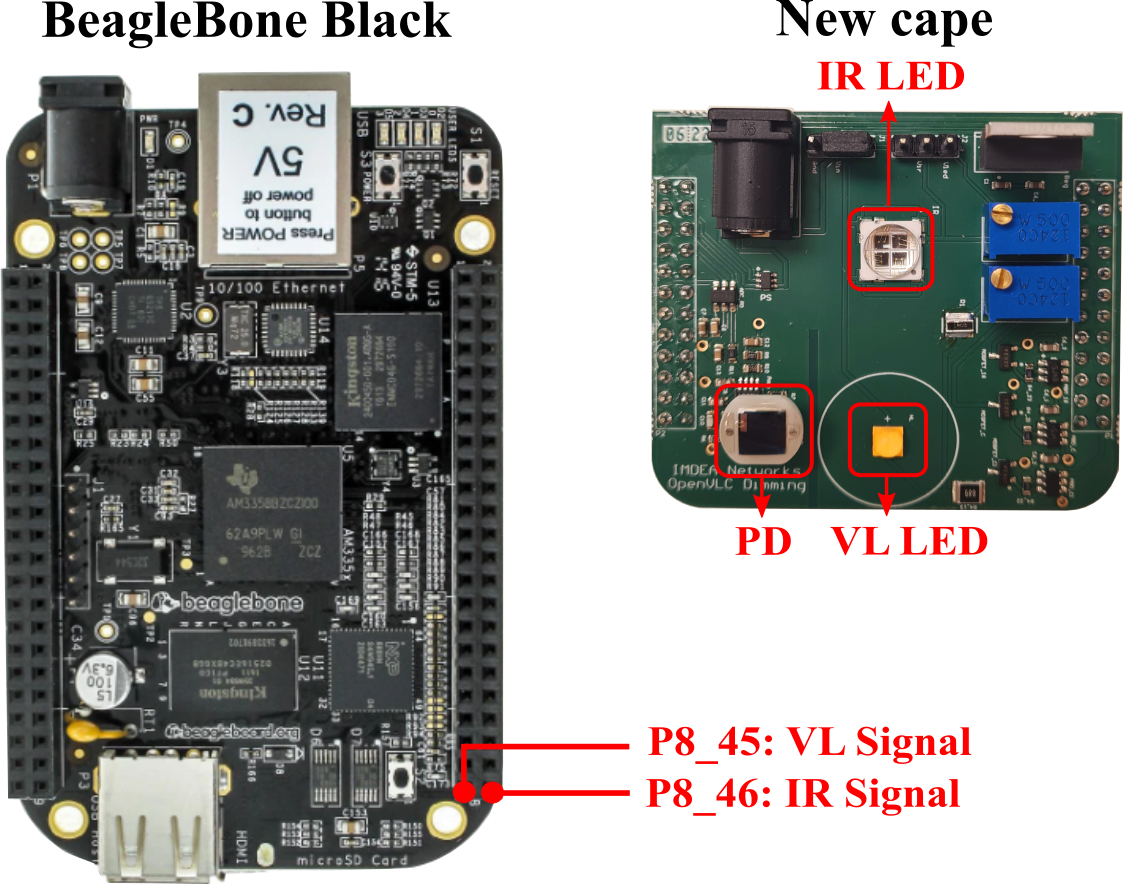
\includegraphics[width=0.9\columnwidth]{openvlc/Cape_for_TX_in_VL_IR_bands}
    \caption{Test iperf riportato nella documentazione di OpenVLC}
    \label{fig:beaglebone_cape}
\end{figure}

Durante la configurazione, sulle schede BeagleBone, viene installato il sistema operativo \textit{Debian 8 "jessie"}. Il driver di OpenVLC è di fatto un modulo del kernel \textit{Linux} che agisce da ponte tra lo stack di rete del sistema operativo e l'hardware BeagleBone.

\paragraph{Reti e Sicurezza.}
Una volta configurate correttamente due schede, la prima come trasmettitore e la seconda come ricevitore, è quindi possibile usarle come una \textit{common network interface}. Ovvero il sistema operativo, in questo caso Debian 8, può usare OpenVLC allo stesso modo in cui userebbe una normale interfaccia di rete, come ad esempio inviare/ricevere pacchetti IP e comunicare con altri dispositivi su una rete locale.\\
Come già anticipato, ognuna delle due schede ha uno ed un solo ruolo, non è infatti possibile attualmente trasmettere e ricevere dalla stessa scheda contemporaneamente. Questo tipo di canale di comunicazione viene denominato \textit{simplex} (unidirezionale), in contrapposizione ad esempio ad un canale \textit{duplex} in cui un device può cambiare ruolo dinamicamente o ad un canale \textit{full-duplex} in cui un device può trasmettere e ricevere simultaneamente.\\
In OpenVLC, per cambiare il ruolo di un device, bisogna di fatto ricompilare il driver.

OpenVLC, essendo un progetto di piccole dimensioni ed avendo come obbiettivo quello di sperimentare con la \gls{vlc}, piuttosto che usarla per comunicazioni realistiche, non implementa delle vere e proprie reti o un infrastruttura hardware/software che permetta di implementare delle reti di calcolatori.

Per quanto riguarda invece la sicurezza, il driver di OpenVLC, gestendo i livelli \gls{phy} e \gls{mac}, non implementa alcun meccanismo di sicurezza. Lascia invece che questa sia gestita dai livelli superiori. Tuttavia definire protocolli di sicurezza a livello fisico è decisamente utile, in particolar modo se si considera che la \gls{vlc} viene utilizzata in contesti in cui la sicurezza delle reti di comunicazione è critica, come ad esempio ospedali e convogli di veicoli.

In figura \ref{fig:design_openvlc} si riporta uno schema riassuntivo dell'architettura di OpenVLC in cui si può osservare quanto descritto precedentemente.
\begin{figure}[H] 
    \centering 
    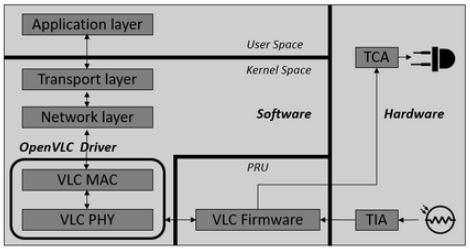
\includegraphics[width=0.9\columnwidth]{openvlc/design_openvlc}
    \caption{Architettura di OpenVLC}
    \label{fig:design_openvlc}
\end{figure}

\paragraph{PHY Frame.}

Come mostrato in figura \ref{fig:phy_frame_structure}, il \gls{phy} frame, cioè la struttura del pacchetto dati a livello fisico, si suddivide in diversi campi.\\
Ogni pacchetto inizia con un preambolo, lungo quattro byte, necessario alla sincronizzazione dei device, a cui segue lo \textit{Start of Frame Delimiter} che indica l'inizio del frame.\\
Successivamente vengono inviati quattro campi da due byte ciascuno: la lunghezza in byte del frame (\textit{Frame Length}), l'indirizzo del device a cui il pacchetto è destinato (\textit{Destination}), l'indirizzo del device da cui proviene (\textit{Source}) e il protocollo di comunicazione (\textit{Protocol}).
A questo punto sono presenti i dati veri e propri, contenuti nel \textit{Payload}, il quale ha una lunghezza variabile da 0 a 255 byte.
Infine, nel campo \textit{Error Correction Code}, si hanno 16 byte necessari alla correzione degli errori generati da Reed-Solomon.
\begin{figure}[H] 
    \centering 
    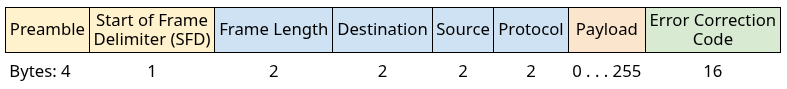
\includegraphics[width=0.9\columnwidth]{openvlc/phy_frame_structure}
    \caption{Struttura del PHY frame in OpenVLC}
    \label{fig:phy_frame_structure}
\end{figure}

\paragraph{Modulazione e Codifica.}
\noindent Come definito dallo standard \gls{ieee} 802.15.7, OpenVLC utilizza la modulazione \gls{ook}\glsfirstoccur nella trasmissione dei dati. In \gls{vlc}, la modulazione dei dati riguarda il modo in cui le informazioni digitali vengono convertite in un segnale analogico tramite la variazione dell'intensità luminosa. In pratica i dispositivi trasmettono bit mediante uno sfarfallio del LED impercettibile all'occhio umano. Si ricorda infatti che lo scopo primario del LED è l'illuminazione, di conseguenza è necessario che rimanga costantemente acceso e che questo sfarfallio sia impercettibile in modo tale da non essere fastidioso per gli occhi.\\
In \gls{vlc}, la modulazione \gls{ook}, è la forma più semplice di modulazione ASK (Amplitude Shift Keying), la quale rappresenta i dati digitali come presenza o assenza di un segnale luminoso che vengono interpretate rispettivamente come bit-1 e bit-0. Questa modulazione è facile da implementare ed ha un basso costo computazionale, tuttavia richiede una sincronizzazione molto precisa tra trasmettitore e ricevitore.

Al fianco della modulazione \gls{ook}, viene usata la codifica \textit{Manchester}, una forma di comunicazione dati nella quale ogni punto viene segnalato da una transizione. Ad esempio, la transizione del segnale, in questo caso luminoso, da basso ad alto viene interpretato dall scheda ricevente come bit-1; viceversa da alto a basso viene interpretato come un bit-0.\\
Nella \gls{vlc} ha il vantaggio di mantenere il bilanciamento DC, riducendo il rischio di \textit{flickering} (sfarfallio) visibile e migliora la sincronizzazione tra trasmettitore e ricevitore.
In OpenVLC l'unico campo del \gls{phy} frame in cui non viene applicata la codifica Manchester è il preambolo, che di conseguenza viene trasmesso in semplice \gls{ook}.

\paragraph{Correzione degli Errori.}
In OpenVLC, la correzione degli errori è gestita tramite i codici Reed-Solomon, ovvero codici di correzione degli errori applicati a livello fisico nella \gls{vlc} per migliorare l'affidabilità della comunicazione e compensare gli errori introdotti da disturbi ambientali.\\
Sia k il numero di byte informativi ed n il numero di byte totali trasmessi, Reed-Solomon RS(n,k) è in grado di correggere fino a (n-k)/2 byte errati.

Nel caso di OpenVLC viene usato RS(216,200), di conseguenza vengono aggiunti 16 byte di correzione degli errori per 200 byte informativi. RS(216,200) non possiede una grandissima capacità di correzione degli errori, ma essendo OpenVLC orientato alla velocità piuttosto che all'affidabilità, riduce sicuramente latenza ed overhead rispetto a varianti di Reed-Solomon più performanti.

\paragraph{Configurazione.}
I dettagli su come è stato configurato il sistema in questo progetto, sulle problematiche riscontrate e su come sono state risolte, si possono trovare nell'appendice \ref{app:A}.


% ================================================================= %
\section{Vulnerabilità}
% possibili attacchi e Vulnerabilità
% cosa assumi sull'attaccante: posizione buona per intercettare il fascio, rubare i pacchet-
% ti, rubare le password, modificare pacchetti, distruggere pacchetti a caso o mandare
% pacchetti a caso

Di seguito vengono elencate le principali vulnerabilità individuate della \gls{vlc}, ed in particolare di OpenVLC, che come menzionato precedentemente non presenta alcun meccanismo di sicurezza, essendo una piattaforma sperimentale ed orientata alla velocità.

\begin{itemize}
    % risolvibili da autenticazione
    \item \textbf{Injection di pacchetti.} In assenza di autenticazione, un dispositivo non autorizzato può trasmettere pacchetti arbitrari sulla rete VLC, simulando il comportamento di un nodo legittimo e causando malfunzionamenti o attacchi di spoofing.
    \item \textbf{Replay di messaggi.} Senza meccanismi di autenticazione e protezione, è possibile catturare e ritrasmettere pacchetti validi, inducendo il ricevitore ad accettare messaggi duplicati o obsoleti.
    % risolvibile da MIC
    \item \textbf{Man-in-the-Middle (MitM).} Un attaccante può inserirsi tra trasmettitore e ricevitore, modificando i pacchetti in transito o iniettando messaggi malevoli, compromettendo l'integrità e l'autenticità della comunicazione.
    % risolvibile da confidenzialità
    \item \textbf{Intercettazione del segnale ottico.} Un attaccante posizionato in modo opportuno può intercettare il fascio luminoso trasmesso tra i dispositivi, acquisendo i pacchetti scambiati e potenzialmente informazioni sensibili come password o dati privati. Come si osserverà dai risultati dei test nel capitolo \ref{cap:test}, considerando che la luce visibile non si propaga in maniera totalmente unidirezionale, questo tipo di attacco non è una possibilità remota, nel momento in cui l'attaccante ha accesso all'ambiente in cui avviene la comunicazione.
    % irrisolvibile se l'attaccante ha accesso al luogo della comunicazione, oppure con codici di correzione molto potenti
    \item \textbf{Distruzione o alterazione dei pacchetti.} Un attaccante può disturbare la comunicazione inviando segnali ottici che interferiscono con la trasmissione, causando la perdita o la corruzione dei dati.
\end{itemize}

\noindent Queste vulnerabilità sono particolarmente rilevanti in contesti in cui la sicurezza della rete è critica, come ambienti industriali, ospedalieri o automotive. L'autenticazione a livello fisico dei messaggi, come proposto nella sezione successiva, permette di mitigare efficacemente tali minacce, garantendo che solo i dispositivi autorizzati possano trasmettere e ricevere pacchetti validi e riducendo il rischio di attacchi di spoofing, MitM e injection.

% ================================================================= %
\section{Soluzione proposta}
% TODO dire che man in the middle e difficile con VL perche' richiede accesso fisico e comunque viene trattato negli sviluppi fututi (MIC)

Per far fronte a tali Vulnerabilità, la soluzione che si propone è l'autenticazione a livello fisico dei messaggi. L'idea di fondo è di fare in modo che il device trasmettitore incorpori nei suoi segnali fisici una \gls{otp} derivata da una \gls{psk}. Il device ricevitore rileva tale \gls{otp}, la estrae dai segnali fisici e la verifica, autenticando, se risulta valida, il device trasmettitore. Se invece non viene rilevata una \gls{otp} valida, il pacchetto viene scartato prima di ulteriori elaborazioni.

La \gls{psk} è una chiave segreta condivisa tra i due dispositivi prima dell'inizio della comunicazione. Può essere condivisa attraverso un canale di comunicazione sicuro, oppure, come nel caso di questo progetto, può essere \textit{"hard-coded"}, cioè codificata direttamente nel codice sorgente dei dispositivi.



% spiega come funziona l'autenticazione a livello fisico.
% vantaggi della soluzione proposta
    \chapter{Progettazione ed implementazione}
\label{cap:progettazione}

\intro{Breve introduzione al capitolo}\\

% ================================================================= %
\section{Progettazione}
% vedi phyauth fine cap 3 (workflow e design)
% motivazioni e progettazione

% ================================================================= %
\section{Implementazione}
% spiega tutto quello che hai fatto testbed codice modificato (motivazione scelte)






Tutte le modifiche apportate sono tracciate nella repository del progetto nel branch PhyAuthP2P: \cite{site:openvlc-pa-github}.
    \chapter{Test e validazione}
\label{cap:test}

\intro{In questo capitolo si espongono e discutono i test svolti su OpenVLC e sul modulo di autenticazione sviluppato. Il capitolo viene diviso in due sezioni: la prima riguarda i test svolti sul modulo di autenticazione sviluppato; la seconda riguarda test generici sul framework OpenVLC.}\\

% ================================================================= %
\section{Test sul modulo di autenticazione}
In questa sezione si riportano i risultati dei test svolti sul modulo di autenticazione sviluppato. L'obbiettivo di questi test è quello di analizzare le prestazioni di OpenVLC con l'utilizzo del modulo, confrontandole con quelle del framework OpenVLC originale. In più, si testa la qualità della comunicazione in diverse condizioni di luminosità ambientale: ambiente luminoso, ambiente buio e ambiente luminoso con disturbo indotto.

Sono stati condotti quattro test, ognuno della durata di circa 30 secondi. In tutti i test le schede sono state posizionate una di fronte all'altra ad una distanza di 100 centimetri. La comunicazione è stata testata utilizzando il comando \texttt{iperf}, il quale è un programma di misurazione delle prestazioni di rete. Si è scelto di utilizzare questo strumento anche per essere paragonabile ai test riportati nella documentazione di OpenVLC, anch'essi svolti con \texttt{iperf}.

In particolare, i comandi utilizzati per i test sono gli stessi riportati nella documentazione ufficiale di OpenVLC: per il trasmettitore "\texttt{sudo iperf -c 192.168.0.2 -u -b 400k -l 800 -p 10001 -t 100}"; mentre per il ricevitore "\texttt{sudo iperf -u -l 800 -s -i3 -B 192.168.0.2 -p 10001}".

\subsection{Data collection}

In figura \ref{fig:iperf_openvlc_originale}, si riporta il test iperf della documentazione di OpenVLC.
\begin{figure}[H] 
    \centering 
    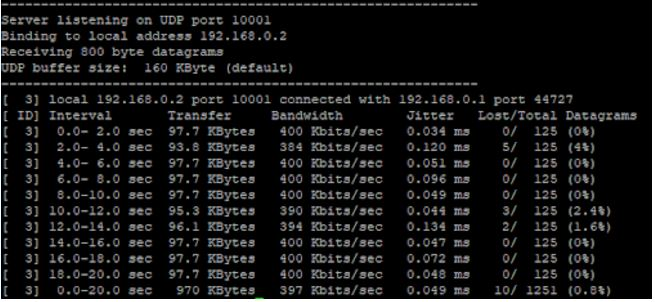
\includegraphics[width=0.9\columnwidth]{test/iperf_openvlc_originale} 
    \caption{Test iperf riportato nella documentazione di OpenVLC}
    \label{fig:iperf_openvlc_originale}
\end{figure}

\noindent In figura \ref{fig:iperf_openvlc_luce_ambiente}, si riporta il test iperf svolto in ambiente luminoso con OpenVLC originale. Si osserva che le differenze rispetto al test illustrato precedentemente, non sono statisticamente significative.
\begin{figure}[H] 
    \centering 
    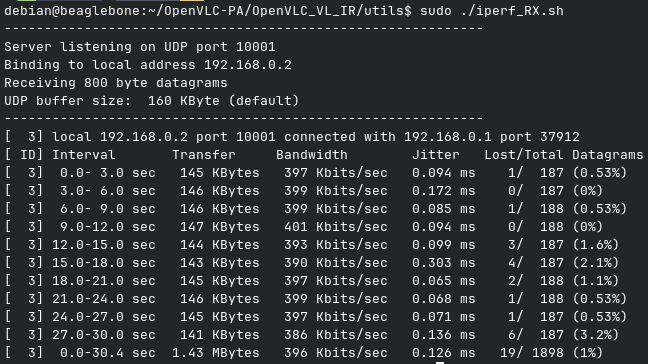
\includegraphics[width=0.9\columnwidth]{test/master_luce_ambiente} 
    \caption{Test iperf con OpenVLC in ambiente luminoso}
    \label{fig:iperf_openvlc_luce_ambiente}
\end{figure}

\noindent In figura \ref{fig:iperf_openvlc_auth_luce_ambiente}, si riporta il test iperf svolto in ambiente luminoso con OpenVLC e con l'utilizzo del modulo di autenticazione sviluppato.
\begin{figure}[H] 
    \centering 
    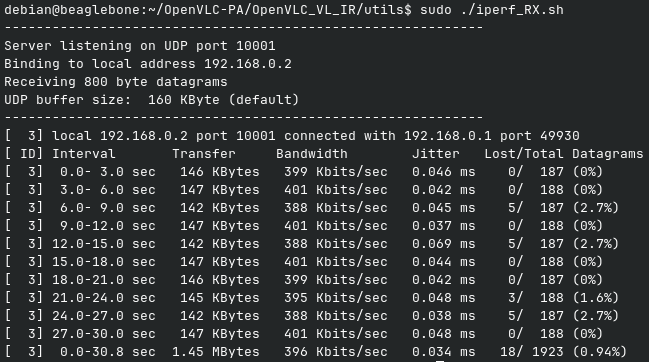
\includegraphics[width=0.9\columnwidth]{test/PhyAuth_luce_ambiente} 
    \caption{Test iperf con OpenVLC e modulo di autenticazione in ambiente luminoso}
    \label{fig:iperf_openvlc_auth_luce_ambiente}
\end{figure}

\noindent In figura \ref{fig:iperf_openvlc_auth_buio}, si riporta il test iperf svolto in ambiente buio con OpenVLC e con l'utilizzo del modulo di autenticazione sviluppato.
\begin{figure}[H] 
    \centering 
    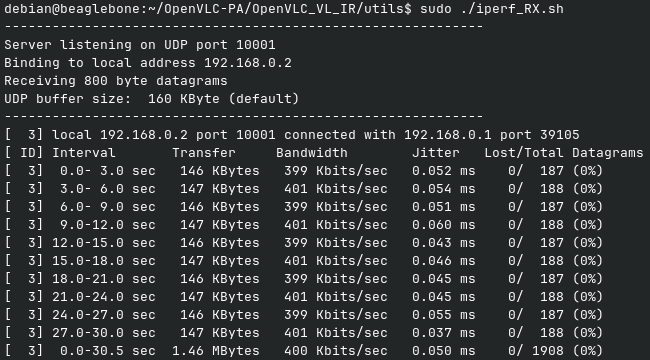
\includegraphics[width=0.9\columnwidth]{test/PhyAuth_buio} 
    \caption{Test iperf con OpenVLC e modulo di autenticazione in ambiente buio}
    \label{fig:iperf_openvlc_auth_buio}
\end{figure}

\noindent In figura \ref{fig:iperf_openvlc_auth_luce_disturbo}, si riporta il test iperf svolto in ambiente luminoso con OpenVLC e con l'utilizzo del modulo di autenticazione sviluppato. In più, in questo test è stato introdotto un disturbo luminoso, posizionando una lampada diretta verso il fotodiodo ricevitore ad una distanza di circa 20 centimetri. Tale disturbo è stato indotto per simulare un attacco di disturbo alla comunicazione, in modo tale da testare la robustezza della comunicazione.
\begin{figure}[H] 
    \centering 
    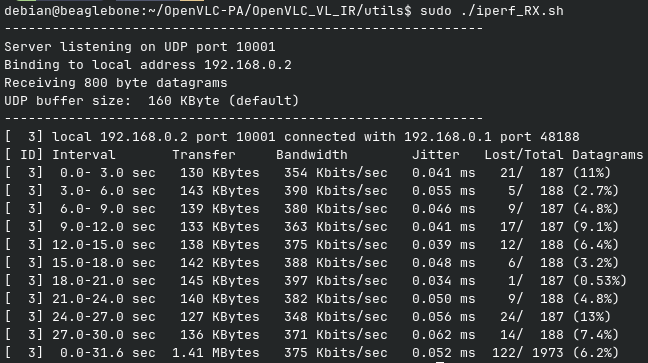
\includegraphics[width=0.9\columnwidth]{test/PhyAuth_luce_e_disturbo} 
    \caption{Test iperf con OpenVLC e modulo di autenticazione in ambiente luminoso con disturbo indotto}
    \label{fig:iperf_openvlc_auth_luce_disturbo}
\end{figure}

\subsection{Analisi dei risultati}

Nella seguente tabella si riassumono i risultati dei test descritti nella precedente sezione. I dati sono ricavati dall'ultima riga di ogni test, che rappresenta il valore medio delle metriche calcolate nell'intervallo di tempo in cui si è svolta la comunicazione.
\begin{table}[H]
    \caption{Tabella riassuntiva dei risultati dei test sul modulo di autenticazione}
    \label{tab:riass-test-auth}
    \resizebox{\textwidth}{!}{%
        \begin{tabular}{llllll}
            \hline
            \textbf{Test} & \textbf{Interval} & \textbf{Transfer} & \textbf{Bandwidth} & \textbf{Jitter} & \textbf{Lost/Total}\\
            \hline
            OpenVLC\\in ambiente\\luminoso & 30.4 sec & 1.43 MBytes & 396 Kbits/sec & 0.126 ms & 19/1898 (1\%) \\
            \hline
            OpenVLC\\+ modulo\\in ambiente\\luminoso & 30.8 sec & 1.45 MBytes & 396 Kbits/sec & 0.034 ms & 18/1923 (0.94\%) \\
            \hline
            OpenVLC\\+ modulo\\in ambiente\\buio & 30.5 sec & 1.46 MBytes & 400 Kbits/sec & 0.050 ms & 0/1988 (0\%) \\
            \hline
            OpenVLC\\+ modulo\\in ambiente\\luminoso\\con disturbo & 31.6 sec & 1.41 MBytes & 375 Kbits/sec & 0.052 ms & 122/1973 (6.2\%) \\
            \hline
        \end{tabular}
    }
\end{table}

\noindent Come si può osservare dalle prime due righe della tabella \ref{tab:riass-test-auth}, a parità di condizioni ambientali, non c'è alcuna differenza sistematicamente significativa tra le prestazioni del sistema con e senza l'utilizzo del modulo di autenticazione. Le lievi differenze presenti sono infatti da interpretarsi come rumore. Di conseguenza si può affermare che la sua introduzione non ha un impatto rilevante sulle prestazioni del sistema.

Si possono invece notare differenze significative tra i test svolti in ambiente luminoso e quelli svolti in diverse condizioni di luminosità.\\
In particolare, il test svolto in ambiente buio ha mostrato un'ampiezza di banda (bandwidth) e un tasso di perdita migliori rispetto a quelli svolti in ambiente luminoso. Questo suggerisce che la comunicazione tramite luce visibile, seppure in maniera minima, trattandosi di una variazione dell'1\%, è sicuramente influenzata dalla presenza di luce ambientale.\\
Inoltre, il test svolto in ambiente luminoso con disturbo indotto ha mostrato un tasso di perdita notevolmente più alto rispetto agli altri test, pari al 6.2\%. Si deduce che la presenza di fonti luminose dirette in direzione del fotodiodo ricevitore, sia in grado di disturbare notevolmente la comunicazione. Tuttavia è importante evidenziare che la situazione in cui è stato testato il sistema, e cioè posizionando una fonte luminosa a distanza molto ravvicinata al fotodiodo, è estrema. Di conseguenza, resta particolarmente difficoltoso, per un potenziale attaccante che volesse disturbare la ricezione dei dati, farlo in questa maniera.

% ================================================================= %
\section{Test su OpenVLC}
In questa sezione si riportano i risultati dei test svolti sul framework OpenVLC originale, cioè senza l'utilizzo del modulo di autenticazione sviluppato. L'obbiettivo di questi test è quello di analizzare le prestazioni di OpenVLC a diverse distanze ed inclinazioni.

Sono stati condotti nove test, in ognuno dei quali sono stati trasmessi 1000 pacchetti di dati tramite il comando \texttt{nc} (netcat), ognuno della dimensione di 1480 byte. In tutti i test il payload era formato da byte "FF", ovvero da 8 bit impostati a "1", in modo tale da poter individuare efficacemente eventuali bit corrotti. L'unica eccezione è il test denominato "50 cm bit-0", in cui il payload era formato da byte "00", ovvero da 8 bit impostati a "0", per poter osservare eventuali bias a favore di bit-0 piuttosto che bit-1.

Tutti i test sono stati svolti in ambiente luminoso e senza l'utilizzo di Reed-Solomon, in modo tale da poter osservare le prestazioni del canale fisico senza l'intervento di alcun protocollo di correzione degli errori.

Inoltre, c'è da precisare che le schede BeagleBone non dispongono di una capacità computazionale elevata, di conseguenza il solo fatto di osservare la comunicazione e salvarne i dati, rende le schede maggiormente soggette ad errori. Questo implica che le metriche di errore calcolate durante i test sono sovrastimate rispetto a quelle che il sistema raggiunge in condizioni normali.\\

\noindent I test vengono valutati utilizzando le seguenti metriche:
\begin{itemize}
    \item \gls{ber}\glsfirstoccur: rapporto tra il numero di bit ricevuti in errore e il numero totale di bit trasmessi, indicativo dell’affidabilità a livello fisico del canale;
    \item Percentuale di byte corrotti: percentuale di byte che contengono almeno un bit errato rispetto al totale dei byte trasmessi, utile per valutare la possibilità di correggere errori con Reed-Solomon;
    \item \gls{prr}\glsfirstoccur: frazione di pacchetti correttamente ricevuti sul numero di pacchetti inviati, misura l’efficacia complessiva del link;
    \item \gls{plr}\glsfirstoccur: percentuale di pacchetti persi rispetto al totale inviato; è il complementare di PRR;
    \item Percentuale di payload ricevuto: rapporto tra il numero di byte di payload validi ricevuti e il numero di byte di payload trasmessi, espressa in percentuale, per quantificare l’efficienza utile della trasmissione.
\end{itemize}

\subsection{Data collection}
Come accennato in precedenza, sono stati condotti nove test, tutti in ambiente luminoso.

L'unico test in cui il payload era formato da byte "00" è il test denominato "50 cm bit-0", in cui le schede sono state posizionate una di fronte all'altra ad una distanza di 50 centimetri. In tutti gli altri il payload era formato da byte "FF".

Nei test denominati "50 cm bit-1", "100 cm", "150 cm", "200 cm", le schede sono state posizionate perfettamente allineate una di fronte all'altra ad una distanza di 50, 100, 150 e 200 centimetri rispettivamente.

Nei test denominati "50 cm 10°", "50 cm 45°", "50 cm 60°", "50 cm 90°", le schede sono state posizionate ad una distanza di 50 centimetri, ma con un'inclinazione di 10°, 45°, 60° e 90° rispettivamente. Ovvero per ogni inclinazione, la scheda trasmittente è stata ruotata, rispetto alla scheda ricevente, di un angolo corrispondente, mantenendo la stessa distanza.

\subsection{Analisi dei risultati}
\subsubsection{Bias a favore di bit-0}
Per prima cosa, è necessario confrontare i test "50 cm bit-0" e "50 cm bit-1", in modo tale da osservare se vi è un bias a favore di bit-0 rispetto a bit-1. In tabella \ref{tab:bit-bias} sono riportate le metriche di errore calcolate per i due test.

Nonostante, a prima vista, la differenza in tutte le metriche sembrerebbe minima, è importante considerare che la numerosità dei campioni è di diversi milioni di bit. Di conseguenza, anche una piccola differenza può essere considerata statisticamente significativa.

Si osserva che le uniche metriche che non presentano una differenza significativa sono il \gls{prr} e il \gls{plr}. Il che denota, come ci si aspetterebbe date le pari condizioni ambientali in cui sono stati svolti i test, che in entrambi i casi le schede riescono a sincronizzarsi correttamente.

Tuttavia, si osserva che il \gls{ber} è più basso per i bit-0 rispetto ai bit-1, con un valore di 1.10\% per i bit-0 e di 1.25\% per i bit-1. Inoltre, la percentuale di byte corrotti è più alta per i bit-1 (2.56\%) rispetto ai bit-0 (1.93\%). Infine, la percentuale di payload ricevuto è più alta per i bit-0 (99.24\%) rispetto ai bit-1 (95.83\%). Questo indica che i bit-1 tendono a essere corrotti più frequentemente rispetto ai bit-0, il che suggerisce un bias a favore dei bit-0.

La presenza di questo bias comporta che le metriche di errore calcolate per i successivi test, in quanto basati su bit-1, sono da considerarsi sovrastimate. In una normale comunicazione, ci si aspetta un bilanciamento tra i bit-0 e i bit-1, e di conseguenza che le metriche di errore siano comprese tra i valori di errore dei bit-0 e dei bit-1 qui presentati.

\begin{table}[H]
    \caption{Confronto delle metriche di errore di bit-0 e bit-1: bias a favore di bit-0}
    \label{tab:bit-bias}
    \begin{tabularx}{\textwidth}{Xll}
        \hline
        \textbf{Metrica} & \textbf{50 cm bit-0} & \textbf{50 cm bit-1}\\
        \hline
        Bit Error Ratio (\gls{ber})            & 1.10\%  & 1.25\% \\
        \hline
        \% Byte corrotti                & 2.56\%  & 1.93\% \\
        \hline
        Packet Reception Rate (\gls{prr})     & 93.80\% & 93.90\% \\
        \hline
        Packet Loss Rate (\gls{plr})          & 6.20\%  & 6.10\% \\
        \hline
        \% Payload Ricevuto             & 99.24\% & 95.83\% \\
        \hline
    \end{tabularx}
\end{table}

\subsubsection{Test in diverse posizioni}
Testando la comunicazione in diverse posizioni, si è osservato che, come ci si aspetterebbe, all'aumentare della distanza e dell'inclinazione tra le schede, tutte le metriche di errore tendono a peggiorare.

In figura \ref{fig:ber_distanze} si riporta il \gls{ber} in funzione della distanza tra le schede. Si osserva una progressiva degradazione della qualità della comunicazione ed un'accelerazione nel tasso di errore a partire dai 100 centimetri.

\begin{figure}[H] 
    \centering 
    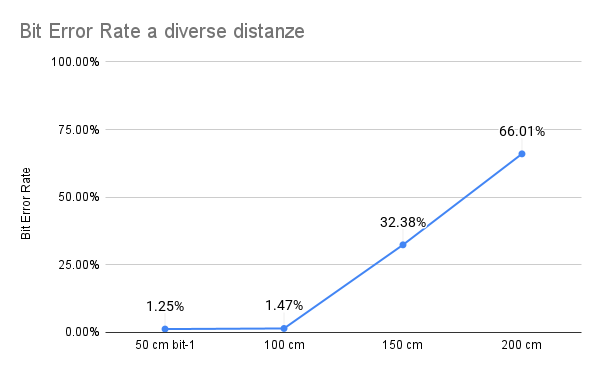
\includegraphics[width=0.9\columnwidth]{test/ber_distanze} 
    \caption{Test \gls{ber} in funzione della distanza}
    \label{fig:ber_distanze}
\end{figure}

Analogamente, in figura \ref{fig:ber_inclinazioni} si riporta il \gls{ber} in funzione dell'inclinazione tra le schede. Anche in questo caso si osserva una degradazione della comunicazione all'aumentare dell'inclinazione, con un tasso di errore che cresce in maniera esponenziale a partire dai 60°.

È interessante notare che, anche ad un'inclinazione ampia come 60°, il BER è comunque limitato. Il che suggerisce che, contrariamente a quanto si potrebbe pensare, la comunicazione tramite luce visibile non sia strettamente unidirezionale, rendendo possibile l'intercettazione del segnale anche da posizioni angolate.\\
Tuttavia, bisogna considerare che i test sono stati svolti ad una distanza limitata, e che combinata a distanze maggiori, l'inclinazione ha sicuramente un impatto negativo sulla comunicazione. Inoltre, come dimostrano i test successivi, all'aumentare dell'inclinazione, corrisponde un aumento del \gls{plr}, il che renderebbe difficoltosa un'intercettazione esaustiva del segnale ad alte inclinazioni.

\begin{figure}[H] 
    \centering 
    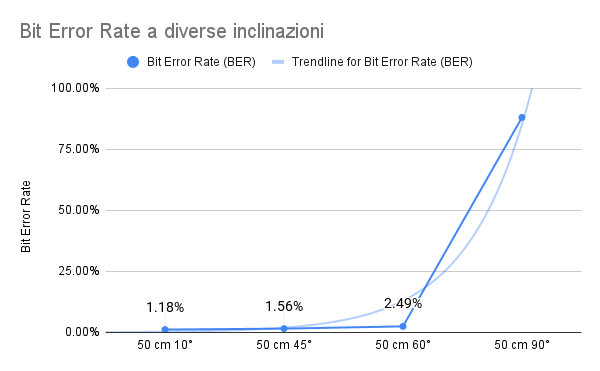
\includegraphics[width=0.9\columnwidth]{test/ber_inclinazioni} 
    \caption{Test Bit Error Ratio (\gls{ber}) in funzione dell'inclinazione}
    \label{fig:ber_inclinazioni}
\end{figure}

In figura \ref{fig:prr_distanze} si riporta il \gls{prr} e la percentuale di payload ricevuto in funzione della distanza tra le schede. Si osserva un graduale peggioramento in entrambe le metriche. Si deduce che, all'aumentare della distanza, aumenta sia la perdita di interi pacchetti, sia la perdita di dati all'interno dei pacchetti stessi. 

\begin{figure}[H] 
    \centering 
    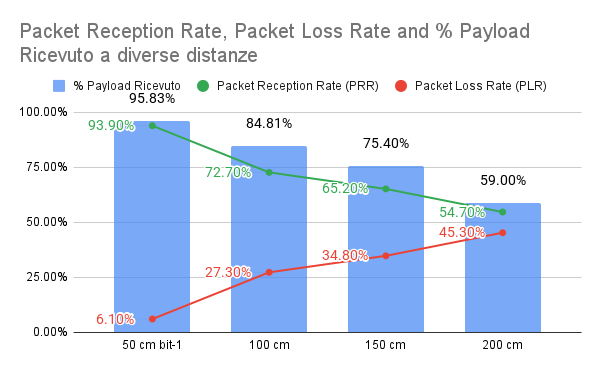
\includegraphics[width=0.9\columnwidth]{test/prr_distanze} 
    \caption{Test Packet Reception Rate (\gls{prr}) in funzione della distanza}
    \label{fig:prr_distanze}
\end{figure}

Analogamente, in figura \ref{fig:prr_inclinazioni} si riporta il \gls{prr} e la percentuale di payload ricevuto in funzione dell'inclinazione tra le schede. Anche in questo caso si possono fare le medesime considerazioni fatte per i test in funzione della distanza.

\begin{figure}[H] 
    \centering 
    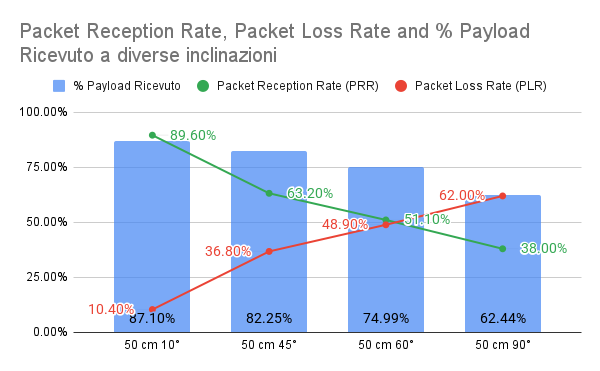
\includegraphics[width=0.9\columnwidth]{test/prr_inclinazioni} 
    \caption{Test Packet Reception Rate (\gls{prr}) in funzione dell'inclinazione}
    \label{fig:prr_inclinazioni}
\end{figure}

In figura \ref{fig:rs_distanze} si riporta la percentuale di byte corrotti in funzione della distanza tra le schede. Inoltre si riportano diversi valori di Reed-Solomon, in modo tale da poter individuare, per ogni distanza, la presenza di un valore di Reed-Solomon che permetta di correggere gli errori a quella distanza.

Ogni valore di Reed-Solomon è indicato da RS(n,k), dove n è il numero di byte totali (informativi + codici di correzione) e k è il numero di byte informativi. Ad esempio RS(15,2) indica un codice Reed-Solomon che per ogni 2 byte di informazione trasmessi, aggiunge 13 byte di codici di correzione, per un totale di 15 byte.\\
Ogni valore di Reed-Solomon è graficamente rappresentato da una \textit{stepped area}, in cui la parte inferiore rappresenta la percentuale di byte che è in grado di correggere. In particolare, sono riportati cinque possibili valori di Reed-Solomon (in ordine di capacità di correzione): RS(15,2), RS(15,4), RS(15,7), RS(15,11) e RS(216,200).\\
Il valore supportato nativamente da OpenVLC è RS(216,200). Gli altri valori sono stati scelti in quanto sono i più diffusi, nonché quelli indicati dallo standard IEEE 802.15.7 per questo tipo di comunicazione\\
Naturalmente, ad una maggiore capacità di correzione corrisponderebbe inevitabilmente un rallentamento nella comunicazione, in quanto si dovrebbero trasmettere più byte di codici di correzione.

Come si può vedere, la percentuale di byte corrotti rispecchia il \gls{ber} e, per distanze fino a 100 centimetri, rientra nelle capacità di correzione di RS(216,200). Questo significa che, come si può osservare empiricamente, a quelle distanze c'è una perdita di informazione molto bassa o addirittura nulla.

\begin{figure}[H] 
    \centering 
    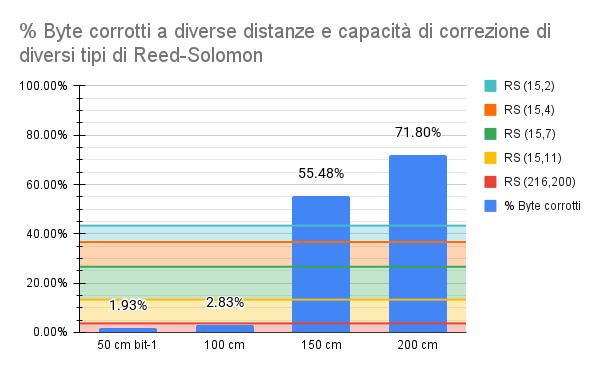
\includegraphics[width=0.9\columnwidth]{test/rs_distanze} 
    \caption{Test sulla percentuale di byte corrotti in funzione della distanza}
    \label{fig:rs_distanze}
\end{figure}

Analogamente, in figura \ref{fig:rs_inclinazioni} si riporta la percentuale di byte corrotti in funzione dell'inclinazione tra le schede. Anche in questo caso si osserva che, fino ad un'inclinazione di 45°, la percentuale di byte corrotti rientra nelle capacità di correzione di RS(216,200). Tuttavia, si può notare che ad una distanza di 60°, per poter garantire la piena correzione degli errori, sarebbe necessario utilizzare un valore di Reed-Solomon più robusto, ad esempio RS(15,11). All'inclinazione di 90°, invece, la percentuale di byte corrotti è tale da non poter essere corretta da alcun valore di Reed-Solomon qui riportato.

\begin{figure}[H] 
    \centering 
    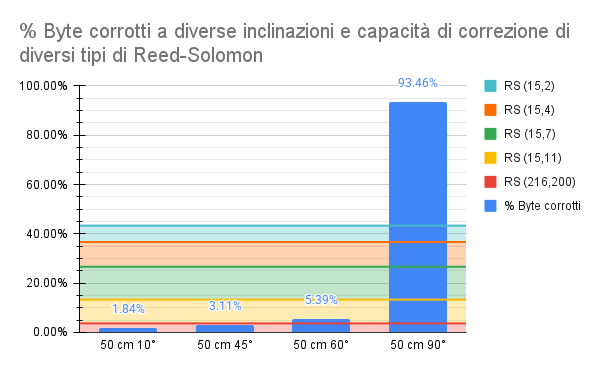
\includegraphics[width=0.9\columnwidth]{test/rs_inclinazioni} 
    \caption{Test sulla percentuale di byte corrotti in funzione dell'inclinazione}
    \label{fig:rs_inclinazioni}
\end{figure}
    \chapter{Conclusioni}
\label{cap:conclusioni}

% ----------------------------------------------------------------- %
\section{Raggiungimento degli obiettivi}

\section{Sviluppi futuri???}

\section{Conoscenze acquisite}

\section{Valutazione personale}


    \appendix
    \chapter{Appendice A}
\label{app:A}

\intro{In questo capitolo si descrive la configurazione del sistema OpenVLC all'interno di questo progetto, si elencano alcune problematiche riscontrate durante la configurazione e il modo in cui sono state risolte.}\\

% ================================================================= %
\section{Configurazione dell'ambiente OpenVLC}

\paragraph{Hardware.} Come indicato nella documentazione OpenVLC, l'hardware necessario comprende unicamente una scheda BeagleBone Black ed un \textit{OpenVLC1.3 RevA cape}.

\paragraph{Software.} La versione di OpenVLC che si è scelto di utilizzare è \textit{OpenVLC 1.3}, in particolare \textit{OpenVLC\_VL\_IR}, in quanto è l'ultima rilasciata ed è compatibile con l'hardware a nostra disposizione.

\paragraph{Configurazione.} Per quanto riguarda la configurazione vera e propria, sono state seguite le istruzioni indicate nella repository ufficiale GitHub di Openvlc: \cite{site:openvlc-github}. Tutte le modifiche alla configurazione originale sono tracciate nella repository del progetto: \cite{site:openvlc-pa-github}.

Per prima cosa si è scritta un'immagine ISO di Debian 8 su una scheda micro SD. Questa immagine contiene una versione di Debian apposita per funzionare su schede BeagleBone.\\
In seguito è necessario installare il sistema operativo sulla scheda BeagleBone. Si è inserita la micro SD nell'apposito slot sulla scheda BeagleBone, e una volta connessa al PC tramite cavo USB e avviata una connessione SSH, si può procedere ad eseguire uno script di installazione.\\
Installato il sistema operativo e riavviata la scheda, è necessario disabilitare l'HDMI in quanto usa alcuni \gls{pru} necessari ad OpenVLC, aggiornare il sistema ed installare gli headers.\\
A questo punto si è incorsi in un errore, in quanto Debian 8, non essendo più supportato, ha archiviato alcune repository. Di conseguenza è stato necessario aggiornarle in modo tale che venissero ricercate nell'archivio.\\
Si deve poi eseguire lo script \textit{load\_test.sh} che compila il driver e permette di cambiare l'indirizzo IP della scheda, è infatti indispensabile che le schede abbiano due indirizzi diversi.\\
L'ultimo passo è quello di configurare il ruolo della scheda (trasmettitore o ricevitore) selezionando lo script corretto all'interno della cartella 'PRU'. In questo progetto, per il trasmettitore, è stato usato \textit{TX\_VL\_IR\_Dimming\_0/deploy.sh} in modo tale da non usare il LED infrarossi, ma solo la luce visibile.

Gli ultimi due passi della configurazione devono essere eseguiti ad ogni avvio della scheda. Per facilitare l'installazione del sistema operativo ed automatizzare l'inizializzazione delle schede sono stati creati alcuni script che si possono trovare nella repository del progetto al percorso \texttt{OpenVLC-PA/OpenVLC\_VL\_IR/utils/}.


    \backmatter
    \printglossary[type=\acronymtype, title=Acronimi e abbreviazioni, toctitle=Acronimi e abbreviazioni]
    \printglossary[type=main, title=Glossario, toctitle=Glossario]

    \cleardoublepage
\chapter{Bibliografia}

\nocite{*}

% Print book bibliography
\printbibliography[heading=subbibliography,title={Riferimenti bibliografici},type=book]

% Print site bibliography
\printbibliography[heading=subbibliography,title={Siti web consultati},type=online]

\end{document}
